%==============================================================================
% Sjabloon poster bachproef
%==============================================================================
% Gebaseerd op document class `a0poster' door Gerlinde Kettl en Matthias Weiser
% Aangepast voor gebruik aan HOGENT door Jens Buysse en Bert Van Vreckem

\documentclass[a0,portrait]{hogent-poster}

% Info over de opleiding
\course{Bachelorproef}
\studyprogramme{Toegepaste Informatica}
\academicyear{2024-2025}
\institution{Hogeschool Gent, Valentin Vaerwyckweg 1, 9000 Gent}

% Info over de bachelorproef
\title{Integratie en vervanging van het DECT-\-systeem met 5G-\-technologie voor zorg-\-simulaties binnen HOGENT}
\author{Maarten Adriaenssens}
\email{maarten.adriaenssens@student.hogent.be}
\supervisor{Lena De Mol}
\cosupervisor{Thomas Cuelenaere (HOGENT), Jens Buysse (CityMesh) en Max Dekoninck (CityMesh)}

% Indien ingevuld, wordt deze informatie toegevoegd aan het einde van de
% abstract. Zet in commentaar als je dit niet wilt.
\specialisation{Systeem- en Netwerkbeheer}
\keywords{Gezondheidszorg, 5G, DECT-systeem, privaat netwerk}
\projectrepo{https://github.com/Maarten-Adriaenssens/latex-hogent-bachproef}

\begin{document}

\maketitle

\begin{abstract}


% It's only a model.
% You don't vote for kings. Who's that then? We found them. Ni! Ni! Ni! Ni!
% The nose? On second thoughts, let's not go there. It is a silly place. Bloody Peasant! And the hat. She's a witch! Where'd you get the coconuts?

Deze bachelorpref onderzoekt de mogelijke communicatietechnologieen die kunnen worden ingezet om het huidige DECT-systeem te vervangen. Doorheen de bachelorproef wordt er zoveel mogelijk rekening gehouden met de huidige noden van de gezondheidszorg. Het doel is om een kwaliteitsvol alternatief te bieden voor de vervanging van het DECT-systeem. Zo wordt er een oplijsting gemaakt van de vereisten en deze afgetoetst met nieuwe technologieën. De technologieën die worden bekeken zijn onder andere: DECT, ULE, VoIP en 5G.
Verder bevat het onderzoek in deze bachelorproef ook een Proof of Concept (PoC) van een 5G netwerk-simulatie, lokaal op de laptop van de student. Deze PoC wordt ook geautomatiseerd en er wordt gekeken naar de mogelijke stappen om deze simulatie om te zetten naar een praktische realisatie.
Uit het onderzoek kan men besluiten dat 5G de beste keuze is op vlak van technologische vervanger van het DECT-systeem. Deze bachelorproef stelt 2 alternatieve opties voor, indien men vandaag een vervanging moet doen met een beperkt budget. De eerste is de nieuwste versie van het DECT-systeem, ook wel het ULE-systeem genoemd. De tweede is een overschakeling naar een combinatie van Wi-Fi en VoIP. Maar in het einde blijft het een afweging tussen de kost en de productiviteitsboost door onder andere de alarmmoeheid vermindering.


\end{abstract}

\begin{multicols}{2} % This is how many columns your poster will be broken into, a portrait poster is generally split into 2 columns

\section{Situering}

Be quiet! Found them? In Mercia?! The coconut's tropical! But you are dressed as one… Well, what do you want? Knights of Ni, we are but simple travelers who seek the enchanter who lives beyond these woods.

Well, what do you want? It's only a model. Camelot! We found them. We shall say `Ni' again to you, if you do not appease us.

The nose? Shut up! Burn her! I am your king. You don't vote for kings.

Why do you think that she is a witch? We want a shrubbery!! I don't want to talk to you no more, you empty-headed animal food trough water! I fart in your general direction! Your mother was a hamster and your father smelt of elderberries! Now leave before I am forced to taunt you a second time!

\section{Proof of Concept}

A newt? Camelot! Why? No, no, no! Yes, yes. A bit. But she's got a wart.

Shut up! I dunno. Must be a king. Who's that then? Look, my liege! On second thoughts, let's not go there. It is a silly place.


\begin{center}
  \captionsetup{type=figure}
  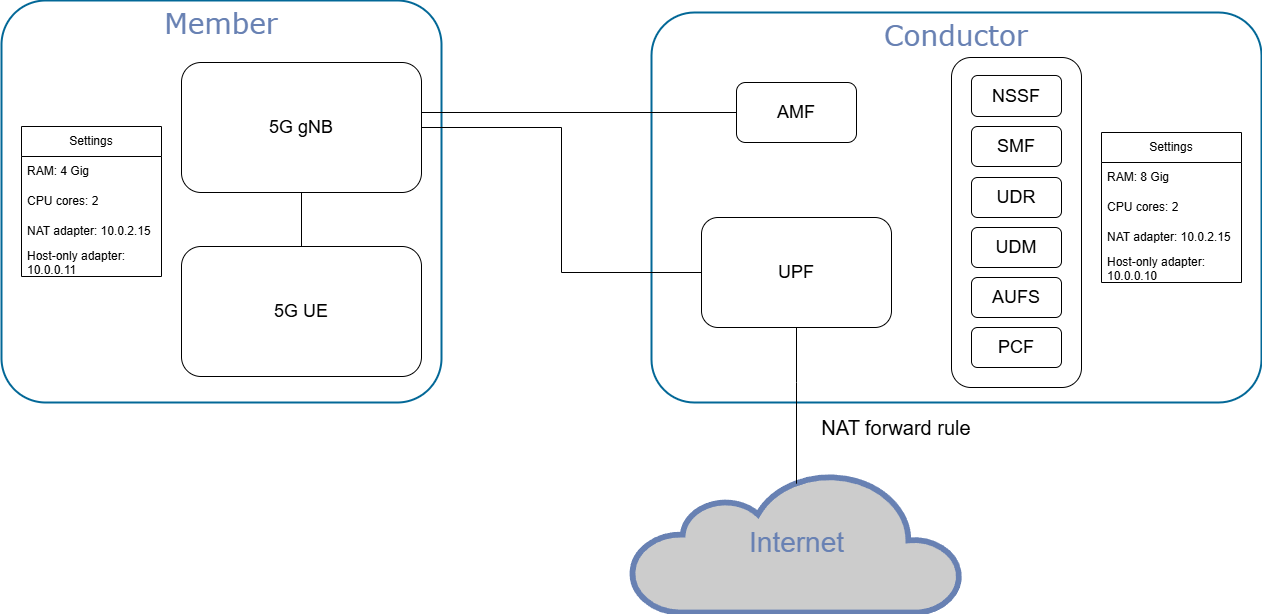
\includegraphics[width=1.0\linewidth]{./graphics/POC-setup.png}
  \captionof{figure}{Proof of Concept Setup}
\end{center}


Shut up! Will you shut up?! No, no, no! Yes, yes. A bit. But she's got a wart. He hasn't got shit all over him. It's only a model. It's only a model.

Bring her forward! I don't want to talk to you no more, you empty-headed animal food trough water! I fart in your general direction! Your mother was a hamster and your father smelt of elderberries! Now leave 

\begin{center}
  \captionsetup{type=figure}
  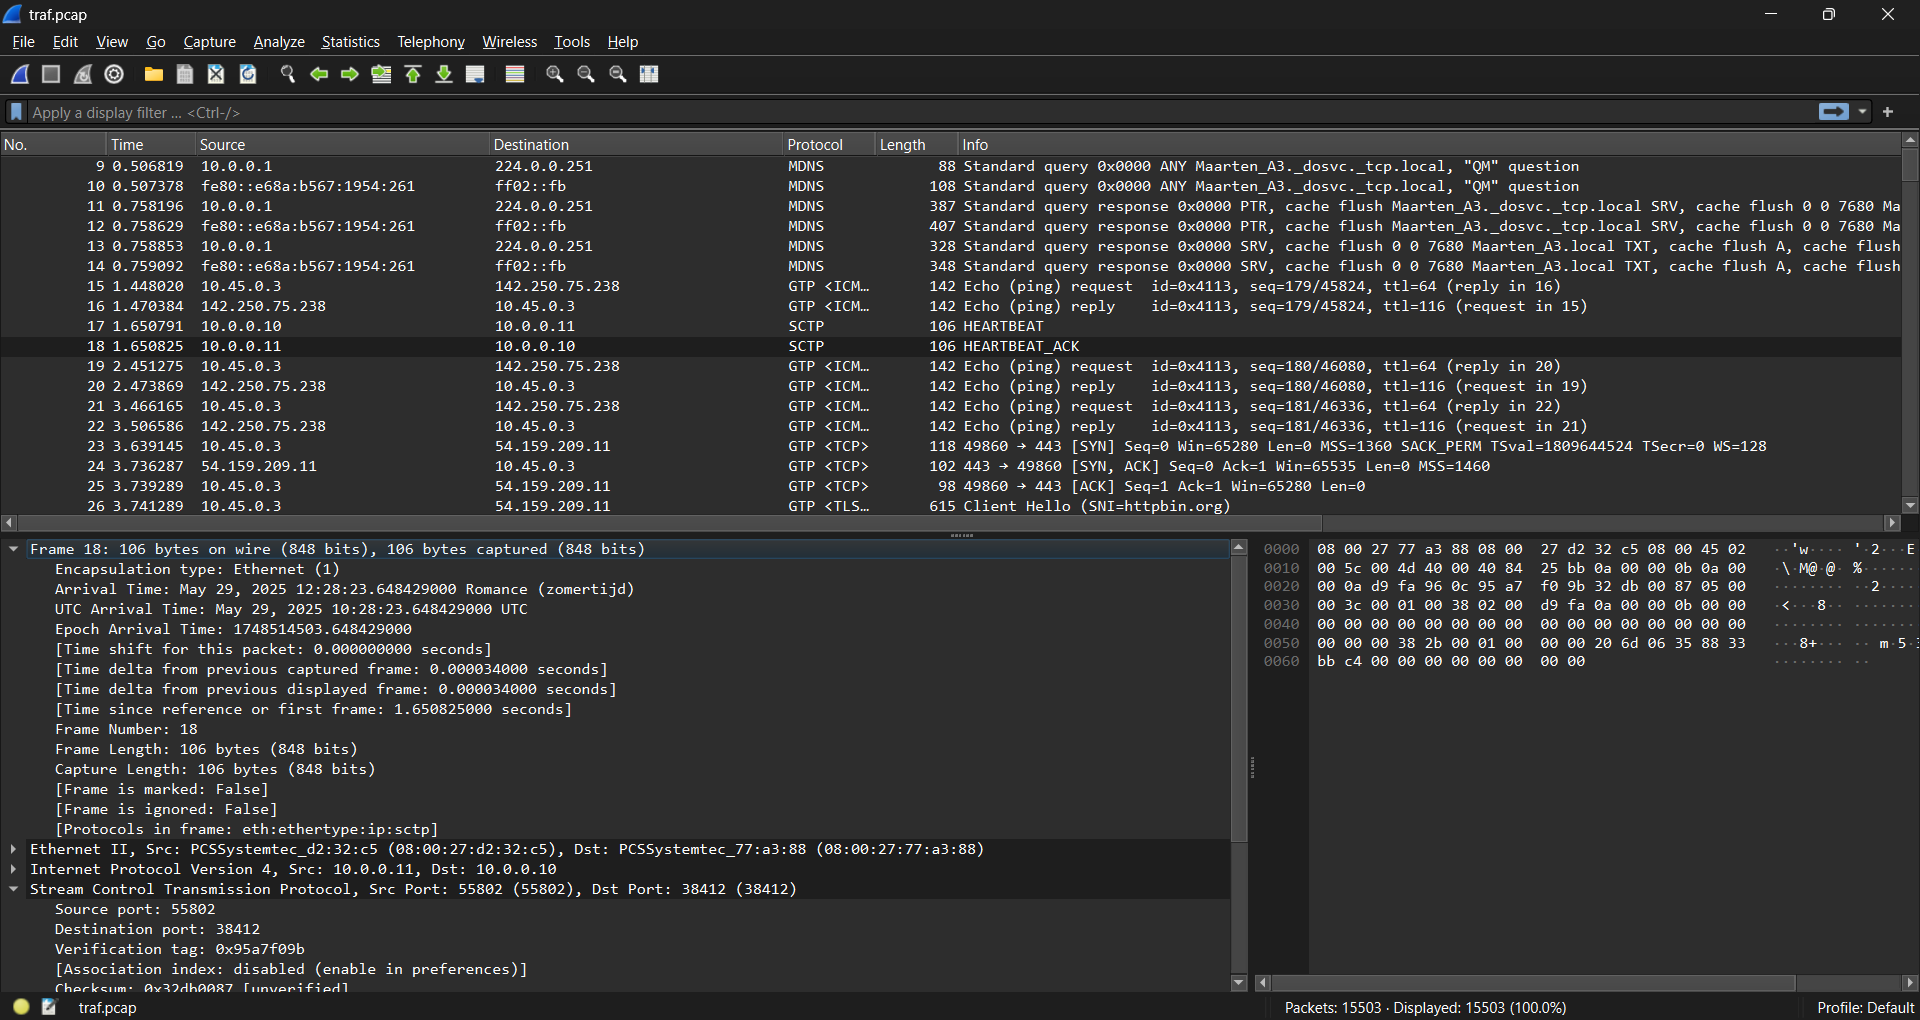
\includegraphics[width=1.0\linewidth]{./graphics/POC-wireshark.png}
  \captionof{figure}{Network capture PoC}
\end{center}


\section{Resultaten}

De {\LaTeX} figure-omgeving bepaalt zelf waar een afbeelding komt en dat is meestal niet op de plek in de tekst waar de figure-omgeving gedefinieerd wordt. Als je wilt forceren dat afbeeldingen toch in de flow van de tekst blijven, dan kan je dat zoals hieronder:

\begin{center}
  \captionsetup{type=figure}
  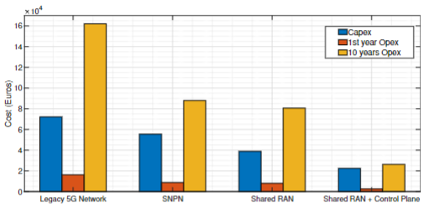
\includegraphics[width=1.0\linewidth]{./graphics/capex-opex.png}
  \captionof{figure}{Capex-Opex vergelijking 5G}
\end{center}

Let er wel op dat dit tot problemen met bladschikking kan leiden.

\section{Conclusies}

Don't underestimate the Force. Oh God, my uncle. How am I ever gonna explain this? I suggest you try it again, Luke. This time, let go your conscious self and act on instinct. Don't be too proud of this technological terror you've constructed. The ability to destroy a planet is insignificant next to the power of the Force.

\section{Toekomstig onderzoek}

Deze bachelorproef dient als springplank voor verder onderzoek en ontwikkeling met als doel het DECT-systeem te vervangen met een kwalitatieve en innovatieve technologie . De eigenschappen van deze technologie hebben als hoofdoel het personeel te ondersteunen en zo de stressfactoren en alamrmoeheid te verminderen of zelfs volledig weg te nemen.

Om dit te testen kan er in de toekomst zeker nog worden samengewerkt met CityMesh en HOGENT. 

\end{multicols}
\end{document}